\documentclass[a4paper, 11pt]{article}

	\usepackage[top=3cm, left=2cm, text={17cm, 24cm}]{geometry}
	\usepackage{color, pict2e, multirow, pdflscape, setspace}
	\usepackage[algo2e, czech, noline, ruled]{algorithm2e}
	\usepackage[unicode, hidelinks]{hyperref}
	\usepackage[utf8]{inputenc}
	\usepackage[czech]{babel}
	\usepackage{times}
	
	\urlstyle{same}

\begin{document}

\begin{titlepage}
	\begin{center}
		{\Huge \textsc{Vysoké učení technické v~Brně}\\}
		{\huge \textsc{Fakulta informačních technologií}\\}
		\vspace{\stretch{0.382}}
		{\LARGE Typografie a~publikování\,--\,3.\ projekt\\}
		{\Huge Tabulky a~obrázky\\}
		\vspace{\stretch{0.618}}
		{\Large \today \hfill Onegen\,Niekto}
	\end{center}
\end{titlepage}

\section{Úvodní strana}

Název práce umístěte do~zlatého řezu a~nezapomeňte uvést \uv{dnešní} (today)
datum a vaše jméno a příjmení.

\section{Tabulky}

Pro sázení tabulek můžeme použít buď prostředí\texttt{ tabbing }nebo
prostředí\texttt{ tabular}.

\subsection{Prostředí\texttt{ tabbing}}

Při použití\texttt{ tabbing }vypadá tabulka následovně:
%
\begin{tabbing}
	Vodni melouny \quad  \= \textbf{Cena} \quad \=                \kill
	\textbf{Ovoce}       \> \textbf{Cena}       \> \textbf{Množství} \\
	Jablka               \> 25,90               \> 3\,kg             \\
	Hrušky               \> 27,40               \> 2,5\,kg           \\
	Vodní melouny        \> 35,--               \> 1\,kus            \\
\end{tabbing}

\noindent
Toto prostředí se dá také použít pro sázení algoritmů, ovšem vhodnější je
použít prostředí\texttt{ algorithm }nebo\texttt{ algorithm2e }(viz sekce
3).

\subsection{Prostředí\texttt{ tabular}}

Další možností, jak vytvořit tabulku, je použít prostředí\texttt{ tabular}.
Tabulky pak budou vypadat takto\footnotemark[1]:

\bigskip
\begin{table}[h!]
	\catcode`\-=12
	\centering
	\begin{tabular}{|l|c|c|}
		\hline
		\multirow{2}{*}{\textbf{Měna}} & \multicolumn{2}{c|}{\textbf{Cena}}                   \\ \cline{2-3}
		                               & \textbf{nákup}                     & \textbf{prodej} \\
		\hline
		EUR                            & 22,705                             & 25,242          \\
		GBP                            & 25,931                             & 28,828          \\
		USD                            & 21,347                             & 23,732          \\
		\hline
	\end{tabular}

	\caption{Tabulka kurzů k~dnešnímu dni}
	\label{tab:kurz}

\end{table}

\bigskip
\begin{table}[h!]
	\catcode`\-=12
	\centering
	\begin{tabular}{|c|c|}
		\hline
		$A$        & $\neg A$ \\
		\hline
		\textbf{P} & N        \\
		\textbf{O} & O        \\
		\textbf{X} & X        \\
		\textbf{N} & P        \\
		\hline
	\end{tabular}
	%
	\begin{tabular}{|c|c|c|c|c|c|}
		\hline
		\multicolumn{2}{|c|}{\multirow{2}{*}{$A \wedge B$}} & \multicolumn{4}{c|}{$B$}                                            \\\cline{3-6}
		\multicolumn{2}{|c|}{ }                             & \textbf{P}               & \textbf{O} & \textbf{X} & \textbf{N}     \\
		\hline
		\multirow{4}{*}{$A$}
		                                                    & \textbf{P}               & P          & O          & X          & N \\ \cline{2-6}
		                                                    & \textbf{O}               & O          & O          & N          & N \\ \cline{2-6}
		                                                    & \textbf{X}               & X          & N          & X          & N \\ \cline{2-6}
		                                                    & \textbf{N}               & N          & N          & N          & N \\ \cline{2-6}
		\hline
	\end{tabular}
	%
	\begin{tabular}{|c|c|c|c|c|c|}
		\hline
		\multicolumn{2}{|c|}{\multirow{2}{*}{$A \vee B$}} & \multicolumn{4}{c|}{$B$}                                             \\\cline{3-6}
		\multicolumn{2}{|c|}{ }                           & \textbf{P}               & \textbf{O} & \textbf{X} & \textbf{N}      \\
		\hline
		\multirow{4}{*}{$A$}
		                                                  & \textbf{P}               & P          & P          & P          & P  \\ \cline{2-6}
		                                                  & \textbf{O}               & P          & O          & P          & O  \\ \cline{2-6}
		                                                  & \textbf{X}               & P          & P          & X          & X  \\ \cline{2-6}
		                                                  & \textbf{N}               & P          & O          & X          & N  \\ \cline{2-6}
		\hline
	\end{tabular}
	%
	\begin{tabular}{|c|c|c|c|c|c|}
		\hline
		\multicolumn{2}{|c|}{\multirow{2}{*}{$A \rightarrow B$}} & \multicolumn{4}{c|}{$B$}                                             \\\cline{3-6}
		\multicolumn{2}{|c|}{ }                                  & \textbf{P}               & \textbf{O} & \textbf{X} & \textbf{N}      \\
		\hline
		\multirow{4}{*}{$A$}
		                                                         & \textbf{P}               & P          & O          & X          & N  \\ \cline{2-6}
		                                                         & \textbf{O}               & P          & O          & P          & O  \\ \cline{2-6}
		                                                         & \textbf{X}               & P          & P          & X          & X  \\ \cline{2-6}
		                                                         & \textbf{N}               & P          & P          & P          & P  \\ \cline{2-6}
		\hline
	\end{tabular}

	\caption{Protože Kleeneho trojhodnotová logika už je \uv{zastaralá},
		uvádíme si zde příklad čtyřhodnotové logiky}
	\label{tab:log}

\end{table}
\bigskip

\footnotetext[1]{
	Kdyby byl problem s\texttt{ cline,} zkuste se podívat třeba sem:
	\url{http://www.abclinuxu.cz/tex/poradna/show/325037}.
}

\pagebreak

\section{Algoritmy}

Pokud budeme chtít vysázet algoritmus, můžeme použít
prostředí\texttt{ algorithm\footnotemark[2] }
nebo\texttt{ algorithm2e\footnotemark[3]}. Příklad použití
prostředí\texttt{ algorithm2e }viz Algoritmus~\ref{alg:fslam}.

\bigskip
\begin{algorithm2e}
	\caption{\textsc{FastSLAM}}
	\label{alg:fslam}

	\LinesNumbered
	\setstretch{0.9}
	\SetInd{1em}{1em}
	\SetNlSty{}{}{:}
	\SetNlSkip{-1.2em}
	\SetArgSty{textrm}
	\SetFuncSty{emph}
	\SetAlgoNlRelativeSize{-1}
	\DontPrintSemicolon

	\SetKwFor{For}{for}{do}{end\ for}
	\SetKwFunction{SampleMotion}{sample\_motion\_model}
	\SetKwFunction{MeasureModel}{measurement\_model}
	\SetKwFunction{UpOccupancy}{$updated\_occupancy\_grid$}

	\KwIn{$(X_{t-1}, u_t, z_t)$}
	\KwOut{$X_t$}
	\Indentp{1.66em}
	\BlankLine

	$\overline{X_t} = X_t = 0$ \;
	\For{$k = 1$ to $M$}{
	$x_t^{[k]} =$ \SampleMotion{$ u_t, x_{t-1}^{[k]} $} \;
	$\omega_t^{[k]} =$ \MeasureModel{$ z_t, x_t^{[k]}, m_{t-1} $} \;
	$m_t^{[k]} =$ \UpOccupancy{$ z_t, x_t^{[k]}, m_{t-1}^{[k]} $} \;
	$\overline{X_t} = \overline{X_t} \; + $
	$\langle x_x^{[m]} , \omega_t^{[m]} \rangle$ \;
	}
	\For{$k = 1$ to $M$}{
	draw $i$ with probability $\approx \omega_t^{[i]}$ \;
	add $\langle x_x^{[k]} , m_t^{[k]} \rangle$ to $X_t$ \;
	}
	\KwRet{$X_t$}
\end{algorithm2e}

\section{Obrázky}

Do~našich článků můžeme samozřejmě vkládat obrázky. Pokud je obrázkem
fotografie, můžeme klidně použít bitmapový soubor. Pokud by to ale mělo
být nějaké schéma nebo něco podobného, je dobrým zvykem takovýto obrázek
vytvořit vektorově.

\begin{figure}[h]
	\centering
	\scalebox{0.4}{
		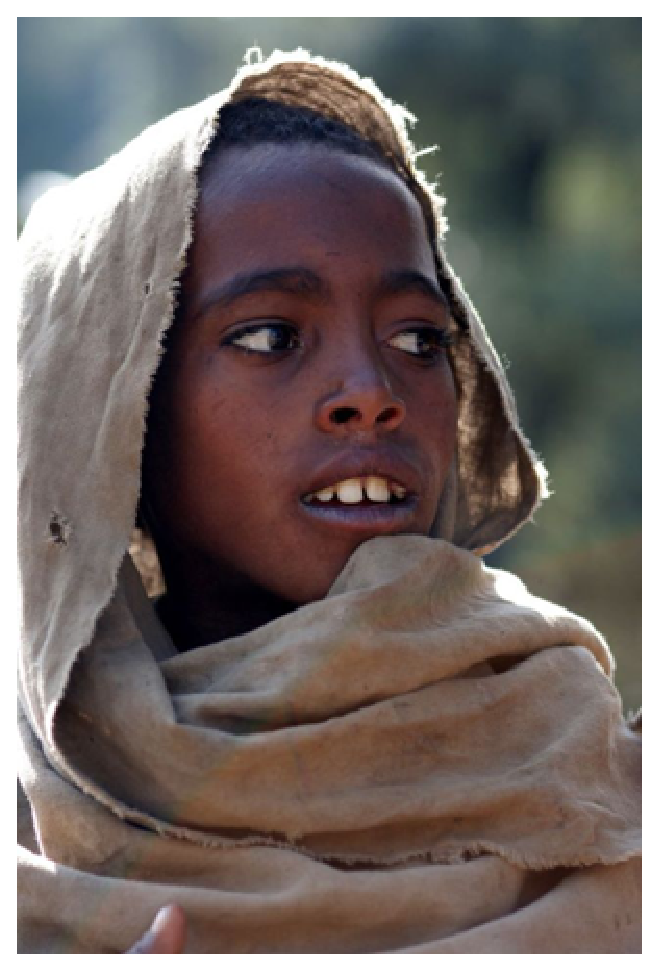
\includegraphics{etiopan.eps}
		\reflectbox{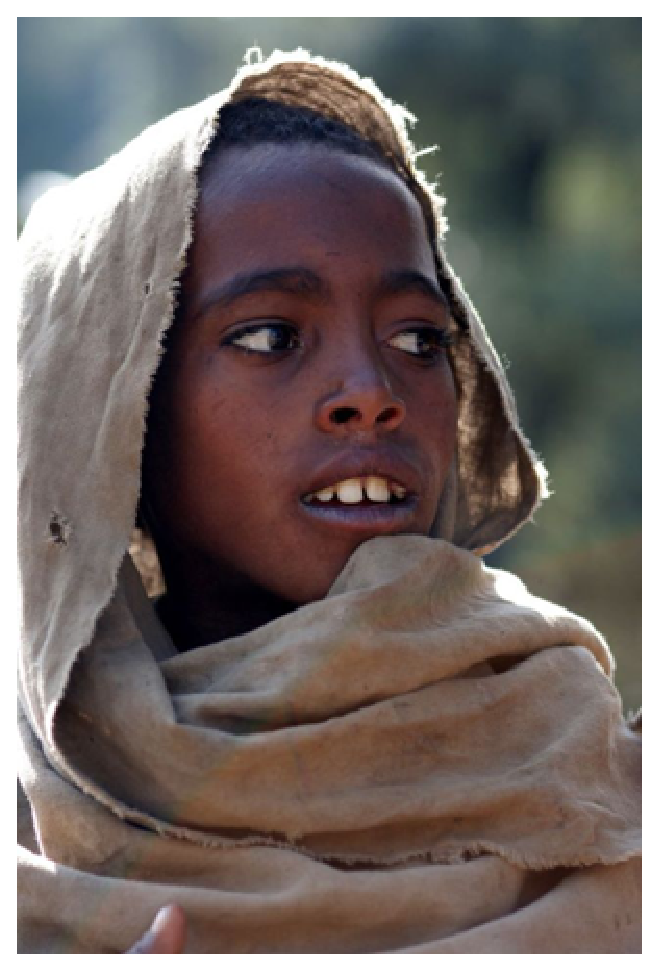
\includegraphics{etiopan.eps}}
	}

	\caption{Malý Etiopánek a~jeho bratříček}
	\label{fig:etiop}
\end{figure}

\footnotetext[2]{
	Pro nápovědu, jak zacházet s~prostředím\texttt{ algorithm,} můžeme
	zkusit tuhle stránku:\\
	\url{http://ftp.cstug.cz/pub/tex/CTAN/macros/latex/contrib/algorithms/algorithms.pdf}.
}

\footnotetext[3]{
	Pro\texttt{ algorithm2e }zase tuhle:
	\url{http://ftp.cstug.cz/pub/tex/CTAN/macros/latex/contrib/algorithm2e/doc/algorithm2e.pdf}.
}

\bigskip
\pagebreak

Rozdíl mezi vektorovým\,\dots

\begin{figure}[h]
	\centering
	\scalebox{0.4}{
		
\includegraphics{oniisan.eps}
	}

	\caption{Vektorový obrázek}
	\label{fig:oniisan}
\end{figure}
\bigskip

\noindent
\dots\,a~bitmapovým obrázkem

\begin{figure}[h]
	\centering
	\scalebox{0.6}{
		
\includegraphics{oniisan2.eps}
	}

	\caption{Bitmapový obrázek}
	\label{fig:oniisan2}
\end{figure}
\bigskip

\noindent
se projeví například při zvětšení.

Odkazy (nejen ty) na obrázky~\ref{fig:etiop},~\ref{fig:oniisan}
a~\ref{fig:oniisan2}, na~tabulky~\ref{tab:kurz} a~\ref{tab:log} a~také
na algoritmus~\ref{alg:fslam} jsou udělány pomocí křížových odkazů. Pak je
ovšem potřeba zdrojový soubor přeložit dvakrát.

Vektorové obrázky lze vytvořit i~přímo v~\LaTeX{}u, například pomocí
prostředí\texttt{ picture.}

\pagebreak
\bigskip

\begin{landscape}
	\begin{figure}[h]
		\centering
		\setlength{\unitlength}{1mm}
		\begin{picture}(200,100)

			% Rám
			\linethickness{2pt}
			\put(0, 0){\framebox(200, 100){}}

			% Pôda a slnko
			\linethickness{4pt}
			\put(5, 5){\line(1, 0){190}}
			\linethickness{0.5pt}
			\put(180, 85){\circle{20}}

			% Dom -- základ
			\linethickness{1pt}
			\put(10, 5){\framebox(110, 7){}}
			\put(10, 12){\framebox(110, 26){}}
			\linethickness{0.5pt}
			\multiput(10, 5)(0, 3.5){2}{\line(1, 0){110}}
			\multiput(15, 5)(10, 0){11}{\line(0, 1){3.5}}
			\multiput(20, 8.5)(10, 0){10}{\line(0, 1){3.5}}

			% Dom -- strecha
			\linethickness{1pt}
			\put(5, 38.2){\line(1, 0){5}}
			\put(120, 38.2){\line(1, 0){5}}
			\put(5, 38.2){\line(1, 2){6}}
			\put(125, 38.2){\line(-1, 2){6}}
			\put(11, 50){\line(1, 50){0.66}}
			\put(119, 50){\line(-1, 50){0.66}}
			\put(11.6, 83){\line(1, 1){10}}
			\put(118.6, 83){\line(-1, 1){10}}
			\put(21.6, 93){\line(1, 0){87}}
			\linethickness{0.5pt}
			\multiput(21, 50)(10, 0){5}{\line(1, 50){0.86}}
			\multiput(69.3, 50)(10, 0){5}{\line(-1, 50){0.86}}
			\multiput(5, 38)(10, 0){6}{\line(1, 2){6}}
			\multiput(75.3, 38)(10, 0){5}{\line(-1, 2){6}}

			% Dom -- miestnosť hore a komín 
			\linethickness{1pt}
			\put(44, 54){\textcolor{white}{\rule{40mm}{15mm}}}
			\put(44, 69.3){\textcolor{white}{\rule{40mm}{12mm}}}
			\put(40, 69.2){\textcolor{white}{\rule{2mm}{3mm}}}
			\put(44, 54){\framebox(40, 15){}}
			\put(40, 69.2){\line(1, 0){4}}
			\put(83, 69.2){\line(1, 0){4}}
			\put(45.8, 81.1){\line(1, 0){35.1}}
			\put(40, 69.2){\line(1, 2){6}}
			\put(86.75, 69.2){\line(-1, 2){6}}
			\put(57, 83){\textcolor{white}{\rule{10mm}{12mm}}}
			\put(57, 83){\framebox(10, 12){}}
			\linethickness{0.5pt}
			\multiput(57, 82.9)(0, 2.5){6}{\line(1, 0){10}}
			\multiput(57, 83)(3.4, 0){3}{\line(0, 1){2.5}}
			\multiput(58.6, 85.5)(3.4, 0){3}{\line(0, 1){2.5}}
			\multiput(57, 88)(3.4, 0){3}{\line(0, 1){2.5}}
			\multiput(58.6, 90.5)(3.4, 0){3}{\line(0, 1){2.5}}
			\multiput(57, 93)(3.4, 0){3}{\line(0, 1){2.5}}

			% Dom -- dvere
			\linethickness{1pt}
			\put(53, 5.66){\textcolor{white}{\rule{25mm}{10mm}}}
			\put(53, 5){\framebox(1.5, 22.9){}}
			\put(76.5, 5){\framebox(1.5, 22.9){}}
			\put(51, 28.1){\line(1, 0){29}}
			\put(54.5, 35.1){\line(1, 0){22.1}}
			\put(51, 28.1){\line(1, 2){3.5}}
			\put(80, 28.1){\line(-1, 2){3.5}}
			\put(58.33, 5){\framebox(14, 20){}}
			\put(65.33, 5){\line(0, 1){20}}
			\linethickness{0.5pt}
			\put(60.6, 12){\framebox(2, 10){}}
			\put(67.66, 12){\framebox(2, 10){}}

			% Dom -- okná
			\linethickness{0.5pt}
			\put(27, 24){\framebox(20, 12){}}
			\put(28, 25){\framebox(18, 10){}}
			\multiput(28, 25)(6, 0){3}{\line(0, 1){10}}
			\put(54, 55.5){\framebox(19, 12){}}
			\put(55, 56.5){\framebox(17, 10){}}
			\put(63.5, 56.5){\line(0, 1){10}}

			% Prístrešok
			\linethickness{1pt}
			\put(120, 33){\line(5, -1){35}}
			\put(120, 25.66){\line(1, 0){35}}
			\put(155, 5){\line(0, 1){21}}
			\put(125, 5){\framebox(25, 14){}}
			\linethickness{0.5pt}
			\multiput(125, 5)(0, 1.77){8}{\line(1, 0){25}}

		\end{picture}
		\caption{Vektorový obrázek mého bydlení vytvořený v~\LaTeX{}u pomocí \texttt{picture}.}
		\label{fig:domov}
	\end{figure}

\end{landscape}

\end{document}
